\chapter{The Query Algebra}
\label{chap:query-algebra}

\begin{aboutchapter}
In this chapter, we formally define a graph query space in terms of subgraph
homomorphisms.
Combined with a set of query operators, this query space forms a graph query
algebra. We show that each operator is well-defined and give a complete set
of operators.
\end{aboutchapter}

\section{Query Results}

\begin{definition}[Database graph]
\label{def:database-graph}
In this thesis, we consider graph databases that are able to store the
information of a directed, labeled and typed multigraph $G$ (loops are allowed).
We call $G$ the database graph and define it as follows:

$G = (V, R, \lambda, \nlabel, \rtype)$, where
\begin{itemize}
  \item $V$ is a finite set of nodes
  \item $R$ is a finite set of relationships
  \item $\nlabels$ is a set of node labels
  \item $\rtypes$ is a set of relationship types
  \item $\lambda : R \rightarrow V \times V$ is a function assigning nodes to
    relationships
  \item $\nlabel ~:~ V \rightarrow \powSet{\nlabels}$ is a function assigning
    labels to nodes
    ($\powSet{X}$ denotes the powerset of a finite set $X$)
  \item $\rtype ~:~ E \rightarrow \rtypes$ is a function assigning relationship
    types to relationships.
\end{itemize}
\end{definition}

\begin{figure}
  \centering
  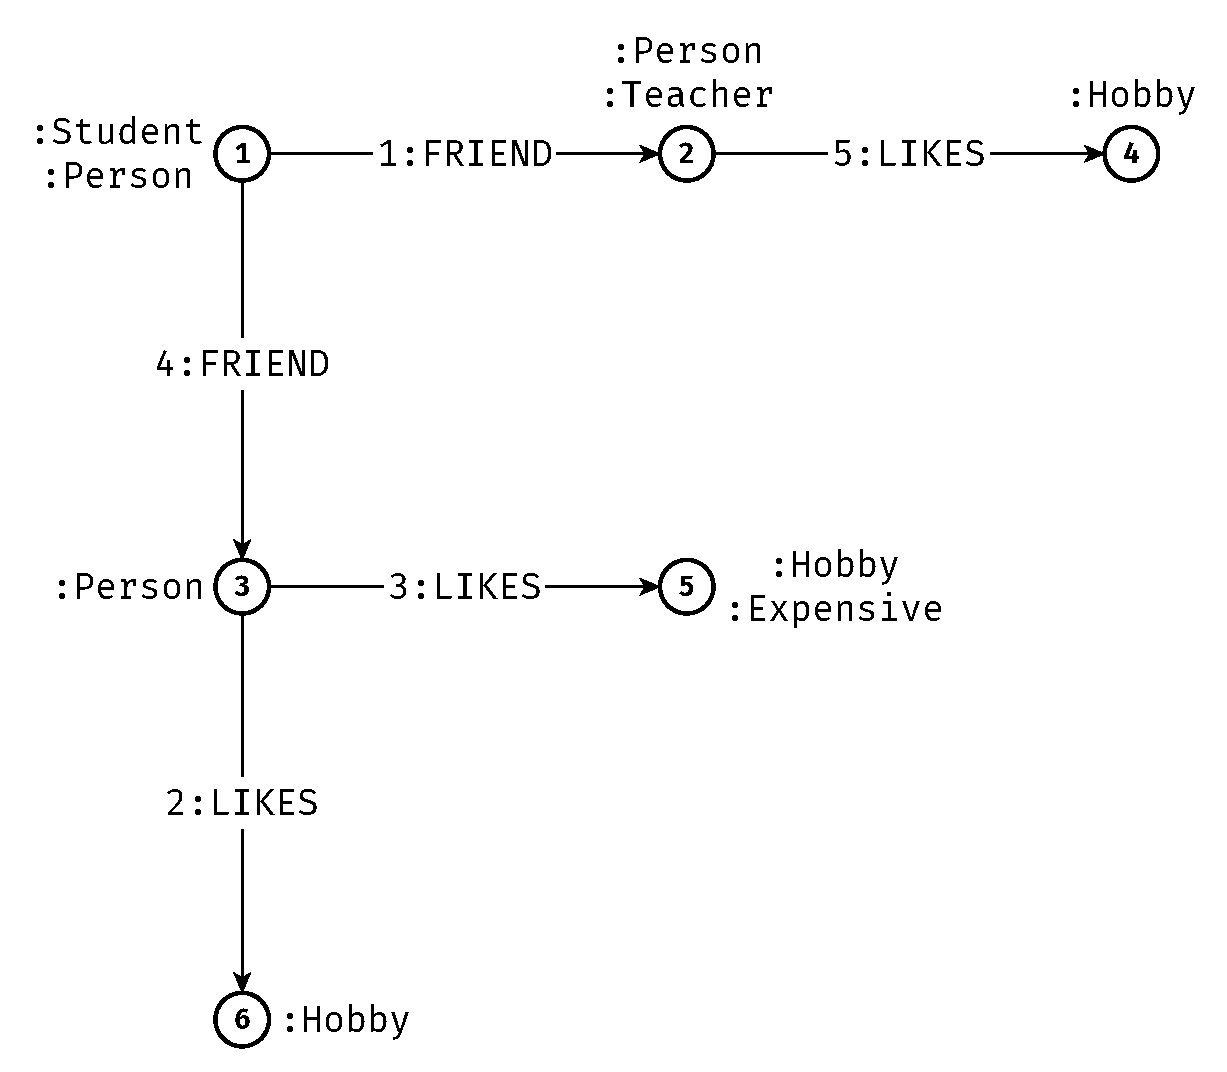
\includegraphics[width=0.7\textwidth]{figures/friend_likes_graph.pdf}
  \caption{A directed, labeled and typed multigraph.}
  \label{fig:dlt-graph}
\end{figure}

Figure \ref{fig:dlt-graph} shows an example database graph from a fictitious
social network. The function $\nlabel$ is encoded by writing all labels from
$\nlabel(v)$ next to the node $v$ in the graph, prefixed by a colon.
The function $\rtype$ is encoded by writing $\rtype(r)$ after each relationship
$r$ in the graph, separated by a colon.
In the example graph, nodes and relationships are identified by natural
numbers. It is required that nodes and relationships are disjoint. Therefore,
we write $x_n$ to refer to the node identified by the number $x$ and $x_r$ to
refer to the relationship identified by $x$.

\begin{remark}
In this thesis, we are only interested in the statistical information
derivable from node labels and relationship types.
We ignore that most graph databases additionally provide
a way of storing properties at nodes.

Node properties can be added to our graph model and to our query
algebra without any interference in the future.
\end{remark}

In a graph database system, queries return sets of subgraphs of the database $G$.
A subgraph can be defined in various ways. In its most general form, a subgraph
is a sequence of nodes of the database, together with a sequence of
relationships between these nodes.
Instead of natural numbers, we use a domain of query variables $\qvars$ to
enumerate the nodes and the relationships.

\begin{definition}[Subgraph]
Consider a domain of query variables $\qvars$. Let $X$ be a finite subset of
this domain.
A subgraph of the database $G$ is a function
$\mu ~:~ X \rightarrow V \union R$
such that
\[
  \forall r \in R ~~ \forall v_1 \in X ~~ (\mu(v_1) = r ~\Rightarrow~
    \exists v_2, v_3 \in X ~~ \lambda(r) = (\mu(v_2), \mu(v_3)))
\]

For $\mu(v) = x$ we say that $x$ is \emph{matched} by the variable $v$ in
the subgraph $\mu$.

We use the following set notation to write a subgraph
$\mu ~:~ \{v_1, \ldots, v_n\} \rightarrow V \union R$:
\[
  \mu = \{ v_1 \mapsto \mu(v_1), v_2 \mapsto \mu(v_2) \ldots, v_n \mapsto \mu(v_n) \}
\]


\end{definition}

In a \emph{query result} we want to collect all subgraphs having a
particular \emph{pattern}.
This pattern is defined as another graph, whose nodes and relationships consist
of query variables. The subgraphs having this pattern are all subgraphs that
are a graph homomorphism from the pattern graph to the database graph.
Our notion of graph homomorphism includes constraints on labels,
relationship types and on relationship uniqueness.

\begin{definition}[Subgraph pattern]
Like the database graph, a subgraph pattern is also a directed, labeled
and typed graph
$\rho = (V_\rho, R_\rho, \lambda_\rho, \nlabel_\rho, \rtype_\rho, \rpairs_\rho)$.

However, $\rtype_\rho$ does not map to one single relationship type,
but to a non-empty set of allowed relationship types:
\[
  \rtype_\rho ~:~ R_\rho \rightarrow \powSet{\rtypes} \setminus \emptyset
\]

Moreover, compared to the database graph, a subgraph pattern has one additional component:
\[
  \rpairs_\rho \subseteq \{ \{r, s\} \mid r,s \in R_\rho \land r \not = s \}
\]
This component will allow us to add uniqueness constraints on pairs of
relationship variables (see Definition \ref{def:query-result}).

Also, both nodes and relationships of a subgraph pattern are finite,
disjoint subsets of a domain of variables $\qvars$:
\begin{enumerate}
  \item $V_\rho \subseteq \qvars$
  \item $R_\rho \subseteq \qvars$
  \item $V_\rho \isect R_\rho = \emptyset$
\end{enumerate}
\end{definition}

The memory requirements of a subgraph pattern are shown in Table
\ref{table:subgraph-pattern-mem-reqs}.

\begin{table}
\centering
\begin{tabular}{ll}
\toprule
Component       & Space complexity                                                    \\ \midrule
$V_\rho$        & $O(\card{V_\rho})$                                                  \\[3pt]
$R_\rho$        & $O(\card{R_\rho})$                                                  \\[3pt]
$\lambda_\rho$  & $O(\card{R_\rho})$                                                  \\[3pt]
$\nlabel_\rho$  & $O(\card{V_\rho} \cdot \card{\nlabels})$                            \\[3pt]
$\rtype_\rho$   & $O(\card{R_\rho})$                                                  \\[3pt]
$\rpairs_\rho$  & $O(\binom{\card{R_\rho}}{2})$                                       \\[3pt]
\textbf{Total:} & $O(\binom{\card{R_\rho}}{2} + \card{V_\rho} \cdot \card{\nlabels})$ \\
\bottomrule
\end{tabular}
\caption{Space complexity of a subgraph pattern.}
\label{table:subgraph-pattern-mem-reqs}
\end{table}

The different components of a subgraph pattern can be best explained by
defining the corresponding query result.

\begin{definition}[Query result]
\label{def:query-result}
The query result $\result(\rho)$ of a subgraph pattern
$\rho = (V_\rho, R_\rho, \lambda_\rho, \nlabel_\rho, \rtype_\rho)$ is defined
as the set of all subgraphs
$\mu ~:~ V_\rho \union R_\rho \rightarrow V \union R$ that fulfil the
following constraints. For all $r,s \in  R_\rho$ and $v, w \in V_\rho$:
\begin{enumerate}[(1)]
  \item Node variables are only mapped to nodes and relationship variables only to relationships:
  
    $\mu(r) \in R$ and $\mu(v) \in V$
  \item Relationships between variables map to relationships in the database:
  
    $\lambda_\rho(r) = (v, w) \Rightarrow \lambda(\mu(r)) = (\mu(v), \mu(w))$
    
  \item The mapped nodes have at least the labels of the variables:
  
    $\nlabel_\rho(v) \subseteq \nlabel(\mu(v))$
    
  \item The mapped relationships are in the set of allowed types for the corresponding variable:
  
    $\rtype(\mu(r)) \in \rtype_\rho(r)$
    
  \item If two relationship variables are marked as disjoint, they map to
    different relationships:
    
    $\{r,s\} \in \rpairs_\rho \Rightarrow \mu(r) \not = \mu(s)$
\end{enumerate}
\end{definition}

\begin{figure}
  \centering
  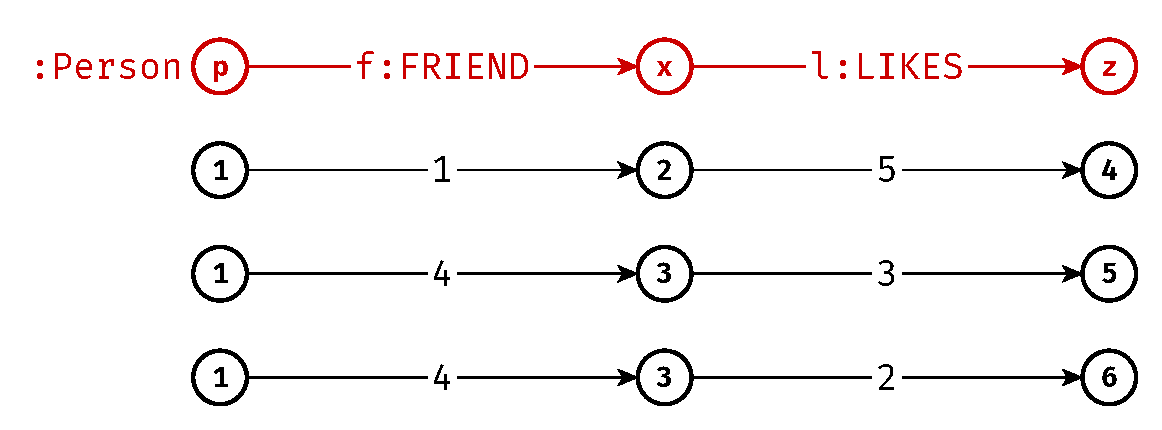
\includegraphics[width=0.7\textwidth]{figures/example-queries/person_p_friend_x_likes_z.pdf}
  \caption{A subgraph pattern and the corresponding query result in the
    database from Figure \ref{fig:dlt-graph}.}
  \label{fig:subgraph-pattern-1}
\end{figure}

Consider the subgraph pattern shown in red in Figure
\ref{fig:subgraph-pattern-1}.
Node and relationship variables are simply drawn from the alphabet.
Each relationship variable is assigned a set of allowed relationship types.
In the given example, these sets happen to consist of only one type.
Semantically, the example subgraph pattern produces all persons having a
friend who likes something. The subgraphs forming the corresponding query
result are shown in black. In set notation, the query result is given as:
\begin{align*}
  \{
    &\{ p \mapsto 1_n, f \mapsto 1_r, x \mapsto 2_n, l \mapsto 5_r, z \mapsto 4_n \} \\
    &\{ p \mapsto 1_n, f \mapsto 4_r, x \mapsto 3_n, l \mapsto 3_r, z \mapsto 5_n \} \\
    &\{ p \mapsto 1_n, f \mapsto 4_r, x \mapsto 3_n, l \mapsto 2_r, z \mapsto 6_n \}
  \}
\end{align*}

Let $\Omega$ be a query result and $\mu \in \Omega$. It is clear that
\[
  V_\rho = \{ v \mid \mu(v) \in V \}
    ~~~~
  R_\rho = \{ r \mid \mu(r) \in R \}
\]
for each subgraph pattern $\rho$ with $\result(\rho) = \Omega$.
This means that all subgraph patterns producing a query result do agree on
the set of node variables and relationship variables.

Therefore we can write these sets of node variables and relationship variables
as functions of $\Omega$:
\[
  \nvars(\Omega) := \{ v \mid \mu(v) \in V \land \mu \in \Omega \}
    ~~~~
  \rvars(\Omega) := \{ r \mid \mu(r) \in R \land \mu \in \Omega \}
\]

For convenience we also define
\[
  \vars(\Omega) := \nvars(\Omega) \union \rvars(\Omega)
\]

\section{The Algebra}
\label{sec:query-algebra}

Now that we have a notion of queries on a graph database (subgraph patterns)
and have defined the corresponding result sets, we are able to introduce a
query algebra.
The query algebra is defined on the space of all query results
\[
  \resultspace := \{ \result(\rho) \mid \rho \text{ is a subgraph pattern} \}
\]

All functions taking a finite number of query results as inputs and producing
another query result as output are possible operators of the algebra:
\[
 \operators := \{ o ~:~ \resultspace^k \rightarrow \resultspace \mid k \in \natnums_0 \}
\]

We will now define a set of operators and show their completeness, i.e., that every
query result can be produced by chaining these operators.

\section{Operators}
\label{sec:operators}

The \op{GetNodes} and \op{Expand} operators were first introduced by
Hölsch et al.\cite{holsch_algebra_2016}.

\begin{definition}[\op{GetNodes} operator]
\label{def:get-nodes}
The \op{GetNodes} operator $\getnodes{v}$ has no inputs and produces the set of
all single node subgraphs of the database $G$.

\begin{align*}
  \getnodes{v} &:= \{ \{ v \mapsto v' \} \mid v' \in V \}
\end{align*}

The subgraph pattern producing $\getnodes{v}$ is trivial:
\[
  \getnodes{v} = \result(
                   \{ v \},
                   \emptyset,
                   \emptyset \rightarrow \{v\}^2,
                   \{ v \mapsto \emptyset \},
                   \emptyset \rightarrow \powSet{\rtypes} \setminus \emptyset,
                   \emptyset)
\]

Therefore $\op{GetNodes}$ is a well-defined operator.
\end{definition}


\begin{definition}[\op{NodeJoin} operator]
\label{def:node-join}
The \op{NodeJoin} operator $\join$ takes two input query results with disjoint relationship variables
and merges them at the overlapping node variables.

Let $\mu_1 \in \Omega_1, \mu_2 \in \Omega_2$, $\rvars(\Omega_1) \isect \rvars(\Omega_2) = \emptyset$.
Merging the subgraphs $\mu_1$ and $\mu_2$ requires that their node matchings
are \emph{compatible} (denoted with $\mu_1 \sim \mu_2$):
\[
  \mu_1 \sim \mu_2 ~~\Leftrightarrow~~ \forall x \in \nvars(\Omega_1) \cap \nvars(\Omega_2): \mu_1(x)=\mu_2(x)
\]
We define the union of these subgraphs as
\[
  (\mu_1 \union \mu_2)(x) := \begin{cases}
                               \mu_1(x), \text{ if } x \in \vars(\mu_1), \\
                               \mu_2(x), \text{ otherwise }
                             \end{cases}
\]

Then we define the node join for all query results $\Omega_1, \Omega_2$
with $\rvars(\Omega_1) \isect \rvars(\Omega_2) = \emptyset$ as:
\begin{align*}
  \Omega_1 \join \Omega_2 &:= \{ \mu_1 \union \mu_2 \mid \mu_1 \in \Omega_1 \land \mu_2 \in \Omega_2 \land \mu_1 \sim \mu_2 \}
\end{align*}

\begin{proofof}{\op{NodeJoin} is a well-defined operator.}
\label{proof:node-join-well-defined}

Let $\Omega_1$ and $\Omega_2$ be query results and
$\rho_1 = (V_{\rho_1}, R_{\rho_1}, \lambda_{\rho_1}, \nlabel_{\rho_1}, \rtype_{\rho_1}, \rpairs_{\rho_1})$, 
$\rho_2 = (V_{\rho_2}, R_{\rho_2}, \lambda_{\rho_2}, \nlabel_{\rho_2}, \rtype_{\rho_2}, \rpairs_{\rho_2})$
be the corresponding subgraph patterns, i.e.
$\Omega_1 = \result(\rho_1)$ and $\Omega_2 = \result(\rho_2)$.

The precondition $\rvars(\Omega_1) \isect \rvars(\Omega_2) = \emptyset$ is
equivalent to $R_{\rho_1} \isect R_{\rho_2} = \emptyset$.

Let then $\rho = (V_\rho, R_\rho, \lambda_\rho, \nlabel_\rho, \rtype_\rho, \rpairs_\rho)$
with
\begin{itemize}[label={}]
  \item $V_\rho := V_{\rho_1} \union V_{\rho_2}$
  \item $R_\rho := R_{\rho_1} \union R_{\rho_2}$
  \item $\lambda_\rho ~:~ R_\rho \rightarrow {V_\rho}^2$ with
    $\lambda_\rho(r) := \begin{cases}
                          \lambda_{\rho_1}(r), \text{ if } r \in R_{\rho_1} \\
                          \lambda_{\rho_2}(r), \text{ if } r \in R_{\rho_2}
                        \end{cases}$
  \item $\nlabel_\rho(v) := L_1 \union L_2$ with
    $L_i := \begin{cases}
              \nlabel_{\rho_i}(v), \text{ if } v \in V_{\rho_i} \\
              \emptyset, \text{ otherwise }
            \end{cases}$ for $i \in \{1,2\}$
  \item $\rtype_\rho(r) := \begin{cases}
                             \rtype_{\rho_1}(r), \text{ if } r \in R_{\rho_1} \\
                             \rtype_{\rho_2}(r), \text{ if } r \in R_{\rho_2}
                           \end{cases}$
  \item $\rpairs_\rho := \rpairs_{\rho_1} \union \rpairs_{\rho_2}$
\end{itemize}

We do now have to show that every subgraph in $\Omega_1 \join \Omega_2$ is also
in $\result(\rho)$ and vice versa.

\begin{itemize}
  \item[$(\subseteq)$]
    Take $\mu \in \Omega_1 \join \Omega_2$. Then $\mu = \mu_1 \union \mu_2$ for
    some $\mu_1 \in \Omega_1$, $\mu_2 \in \Omega_2, \Omega_1 \sim \Omega_2$.
    
    We show that each constraint of Definition \ref{def:query-result} is fulfilled:
    \begin{enumerate}[(1)]
      \item % (1) Relationship variables are mapped to relationships and node variables to nodes
        Take $v \in V_\rho$ arbitrary. If $v \in V_{\rho_1}$ then $\mu(v) = \mu_1(v)$ and
        because $\mu_1 \in \Omega_1$ and $\Omega_1$ is a query result it holds that $\mu_1(v) \in V$.
        Analogously for $v \in V_{\rho_1}$.
        
        Take $r \in R_\rho$ arbitrary. If $r \in R_{\rho_1}$ then $\mu(r) = \mu_1(r)$ and
        because $\mu_1 \in \Omega_1$ and $\Omega_1$ is a query result it holds that $\mu_1(r) \in R$.
        Analogously for $r \in R_{\rho_2}$.
        
      \item % (2) Relationships between variables map to relationships in the database
        Assume $\lambda_\rho(r) = (v, w)$ for some $r \in R_{\rho_1}$ and $v,w \in V_\rho$.
        
        Then $\lambda_\rho(r) = \lambda_{\rho_1}(r) = (v, w)$. Because $\mu_1 \in \result(\rho_1)$
        it follows by constraint (2) that $\lambda(\mu_1(r)) = (\mu_1(v), \mu_1(w))$.
        
        Because $\Omega_1$ and $\Omega_2$ are compatible it holds that $\mu_1(x) = \mu(x)$ for all
        $x \in V_{\rho_1} \union R_{\rho_1}$. Therefore $\lambda(\mu(r)) = (\mu(v), \mu(w))$.
        
        Analogously for $r \in R_{\rho_2}$.
      
      \item % (3) The mapped nodes have at least the labels of the variables
        Take $v \in V_\rho$ arbitrary.
        
        If $v \in V_{\rho_1} \setminus V_{\rho_2}$
        then $\nlabel_\rho(v) = \nlabel_{\rho_1}(v) \subseteq \nlabel(\mu_1(v)) = \nlabel(\mu(v))$.
        
        Analogously for $v \in V_{\rho_2} \setminus V_{\rho_1}$.
        
        If $v \in V_{\rho_2} \isect V_{\rho_1}$
        then $\nlabel_\rho(v) = \nlabel_{\rho_1}(v) \union \nlabel_{\rho_2}(v)
          \subseteq \nlabel(\mu_1(v)) \union \nlabel(\mu_2(v)) = \nlabel(\mu(v))$.
      
      \item % (4) The mapped relationships are in the set of allowed types
        Take $r \in R_\rho$ arbitrary.
        
        If $r \in R_{\rho_1}$ then $\rtype_\rho(r) = \rtype_{\rho_1}(r) \ni \rtype(\mu_1(r)) = \rtype(\mu(r))$.
        
        Analogously for $r \in R_{\rho_2}$.
      
      \item % (5) Relationships are unique in each partition.
        Take $\{r,s\} \rpairs$ arbitrary.
        
        If $\{r,s\} \in \rpairs_{\rho_1}$, then
        $\mu(r) = \mu_1(r) \not = \mu_1(s) = \mu(s)$ because
        $\mu_1 \in \result(\rho_1)$.
        
        Analogously for $\{r,s\} \in \rpairs_{\rho_2}$.
    \end{enumerate}
  
  Therefore $\mu \in \result(\rho)$.
  
  \item[$(\supseteq)$]
    Take $\mu \in \result(\rho)$.
    
    Let $\mu_1 ~:~ V_{\rho_1} \union R_{\rho_1} \rightarrow V \union R$ with $\mu_1(x) := \mu(x)$
    and $\mu_2 ~:~ V_{\rho_2} \union R_{\rho_2} \rightarrow V \union R$ with $\mu_2(x) := \mu(x)$.
    
    Then $\mu_1 \in \result(\rho_1) = \Omega_1$ and $\mu_2 \in \result(\rho_2) = \Omega_2$.
    
    Also $\mu_1 \sim \mu_2$.
    
    Therefore $\mu \in \Omega_1 \join \Omega_2$.
\end{itemize}

We have shown that, for any input results $\Omega_1 = \result(\rho_1)$,
$\Omega_2 = \result(\rho_2)$, there is a subgraph pattern $\rho$ with
$\result(\rho) = \Omega_1 \join \Omega_2$.

Therefore \op{NodeJoin} is a well-defined query operator mapping from
$\resultspace^2$ to $\resultspace$.
\end{proofof}
\end{definition}

\begin{example}
  \newcommand{\pfriendofx}{\vcenter{\hbox{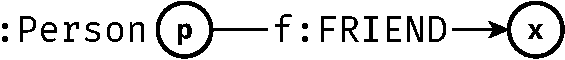
\includegraphics[height=2.6ex]{figures/subgraph-patterns/person_p_friend_x.pdf}}}}
  \newcommand{\xlikesz}{\vcenter{\hbox{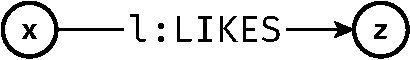
\includegraphics[height=2.6ex]{figures/subgraph-patterns/x_likes_z.pdf}}}}
  \newcommand{\pfriendofxlikesz}{\vcenter{\hbox{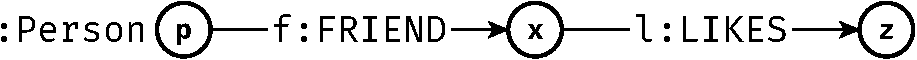
\includegraphics[height=2.6ex]{figures/subgraph-patterns/person_p_friend_x_likes_z.pdf}}}}
  
  It holds that
  \begin{align*}
    &\result(\pfriendofx) \join \result(\xlikesz) \\
    &~~ = \result(\pfriendofxlikesz)
  \end{align*}
\end{example}



\begin{definition}[\op{Traverse} operator]
\label{def:traverse}

The \op{Traverse} operator $\traversevar{v}{r:T}{\alpha}{w}(\Omega)$ takes a query
result $\Omega$ as input and expands it by adding new relationships between nodes.
The precondition is that $v,w \in \nvars(\Omega)$.
The direction of the relationships is specified by
$\alpha \in \{\leftarrow, \rightarrow\}$
and the allowed relationship types by
$T \subseteq \rtypes$.

For $\lambda(s) = (p, q)$ we set $\lambda_\rightarrow(s) = (p, q)$ and
$\lambda_\leftarrow(s) = (q, p)$.

Then we define
\begin{align*}
  \traversevar{v}{r:T}{\alpha}{w}(\Omega) := \{ &\mu \union \{ r \mapsto r' \} \mid
    \mu \in \Omega \land \lambda_\alpha(r') = (\mu(v), \mu(w)) \land t(r') \in T \}
\end{align*}

\begin{proofof}{\op{Traverse} is a well-defined operator.}
\label{proof:traverse-well-defined}

Let $\Omega$ be a query result and
$\rho' = (V_{\rho'}, R_{\rho'}, \lambda_{\rho'}, \nlabel_{\rho'}, \rtype_{\rho'}, \rpairs_{\rho'})$
the corresponding subgraph pattern.

Let then $\rho = (V_\rho, R_\rho, \lambda_\rho, \nlabel_\rho, \rtype_\rho, \rpairs_\rho)$
with
\begin{itemize}[label={}]
  \item $V_\rho := V_{\rho'}$
  \item $R_\rho := R_{\rho'} \union \{ r \}$
  \item $\lambda_\rho(x) := \begin{cases}
                              (v, w) \text{ if } x = r ~\land~ \alpha = \rightarrow \\
                              (w, v) \text{ if } x = r ~\land~ \alpha = \leftarrow \\
                              \lambda_{\rho'}(x), \text{ otherwise}
                            \end{cases}$
  \item $\nlabel_\rho := \nlabel_{\rho'}$
  \item $\rtype_\rho(x) := \begin{cases}
                              T, \text{ if } x = r \\
                              \rtype_{\rho'}(x), \text{ otherwise}
                           \end{cases}$
  \item $\rpairs_\rho := \rpairs_{\rho'}$
\end{itemize}

Again we have to show that every subgraph in
$\traversevar{v}{r:T}{\alpha}{w}(\Omega)$ is also in $\result(\rho)$ and vice
versa.

\begin{itemize}
  \item[$(\subseteq)$]
    Take $\mu \in \traversevar{v}{r:T}{\alpha}{w}(\Omega)$ arbitrary.
    Then $\mu = \mu' \union \{ r \mapsto r' \}$ for some $\mu' \in \Omega$,
    $r' \in R$, such that $\lambda_\alpha(r') = (\mu'(v), \mu'(w'))$.
    
    We show again that each constraint of Definition \ref{def:query-result} is
    fulfilled:
    \begin{enumerate}[(1)]
      \item % (1) Node variables are mapped to nodes and relationship variables
            % to relationships
        $\mu(r) = r' \in R$ by definition.
        For all $v \in V_\rho, s \in R_\rho \setminus \{r\}$:
        $\mu(v) = \mu'(v) \in V$ and $\mu(s) = \mu'(s) \in R$ because
        $\mu' \in \Omega$ and $\Omega$ is a query result.
      \item % (2) Relationships between variables map to relationships in the
            %     database
        If $\alpha = \rightarrow$
        then $\lambda_\rho(r) = (v, w)$
        and $\lambda(\mu(r)) = \lambda(r') = \lambda_\rightarrow(r')
                             = (v', w') = (\mu(v), \mu(w))$.
        
        If $\alpha = \leftarrow$
        then $\lambda_\rho(r) = (w, v)$
        and $\lambda(\mu(r)) = \lambda(r') = \lambda_\rightarrow(r')
                             = (w', v') = (\mu(w), \mu(v))$.
        
        For $x \in R_\rho, x \not = r$ it holds that if
        $\lambda_\rho(x) = \lambda_{\rho'}(x) = (p, q)$
        then $\lambda(\mu(x)) = \lambda(\mu'(x))
                              = (\mu'(p), \mu'(q)) = (\mu(p), \mu(q))$
        because $\mu' \in \Omega$ and $\Omega$ is a query result.
        
      \item % (3) The mapped nodes have at least the labels of the variables
        Take $v \in V_\rho$ arbitrary.
        $\nlabel_\rho(v) = \nlabel_{\rho'}(v) \subseteq \nlabel(\mu'(v))
                         = \nlabel(\mu(v))$.
      
      \item % (4) The mapped relationships are in the set of allowed types
        $\rtype_\rho(r) = T \ni t(r') = t(\mu(r))$ by definition.
        
        For $s \in R_\rho, s \not = r$ it holds that
        $\rtype_\rho(s) = \rtype_{\rho'}(s) \ni \rtype(\mu'(s)) = \rtype(\mu(s))$.
      
      \item % (5) Relationships are mapped different if they are marked different.
        Take $\{s,t\} \in \rpairs_\rho = \rpairs_{\rho'}$ arbitrary.
        Then $s,t \in R_{\rho'}$ and therefore $\mu(s) = \mu'(s)$ and
        $\mu(t) = \mu'(t)$.
        
        Because $\mu' \in \result(\rho')$ it follows that
        $\mu(s) = \mu'(s) \not = \mu'(t) = \mu(t)$.
    \end{enumerate}
    
    As a result, $\mu \in \result(\rho)$.

  \item[$(\supseteq)$]
    Take $\mu \in \Omega = \result(\rho)$ arbitrary. Let
    $\mu' ~:~ V_{\rho'} \union R_{\rho'} \rightarrow V \union R$ with
    $\mu'(x) := \mu(x)$.
    Then $\mu' \in \result(\rho') = \Omega$.
    
    If $\alpha = \rightarrow$
    then $\lambda_\rho(r) = (v, w)$
    and because of constraint (2)
    $\lambda_\alpha(\mu(r)) = \lambda(\mu(r)) = (\mu(v), \mu(w))$.
    
    Analogously for $\alpha = \leftarrow$.
    
    Finally, $\rtype(r') = \rtype(\mu(r)) \in \rtype_\rho(r) = T$.
    
    Therefore, $\mu \in \traversevar{v}{r:T}{\alpha}{w}(\Omega)$.
\end{itemize}

It follows that $\traversevar{v}{r:T}{\alpha}{w}(\Omega) = \result(\rho)$.
We conclude that \op{Traverse} is a well-defined operator.
\end{proofof}
\end{definition}



\begin{definition}[\op{Expand} operator]
\label{def:expand}

The \op{Expand} operator $\expandvar{v}{r:T}{\alpha}{w}(\Omega)$ takes a query
result $\Omega$ as input and expands it by adding new nodes using
relationships. The preconditions are that
$v \in \nvars(\Omega)$
and
$w \not \in \nvars(\Omega)$
The direction of the relationships is specified by
$\alpha \in \{\leftarrow, \rightarrow\}$
and the allowed relationship types by
$T \subseteq \rtypes$.

For $\lambda(r) = (v, w)$ we set $\lambda_\rightarrow(r) = (v, w)$ and
$\lambda_\leftarrow(r) = (w, v)$.

Then we define
\[
  \expandvar{v}{r:T}{\alpha}{w}(\Omega) := \{ \mu \union \{ r \mapsto r', w \mapsto w' \} \mid
                                              \mu \in \Omega \land \lambda_\alpha(r') = (\mu(v), \mu(w))
                                              \land \rtype(r') \in T \}
\]

\begin{proofof}{\op{Expand} is a well-defined operator.}
\label{proof:expand-well-defined}

By definition it holds that
\begin{align}
\begin{split}
  \expandvar{v}{r:T}{\alpha}{w}(\Omega) &= \{ \mu \union \{ r \mapsto r' \} \union \{ w \mapsto w' \} \mid
                                              \mu \in \Omega \land \lambda_\alpha(r') = (\mu(v), \mu(w))
                                              \land \rtype(r') \in T \} \\
                                        &= \{ \mu_1 \union \mu_2 \union \{ r \mapsto r' \} \mid
                                              \mu_1 \in \Omega \land \mu_2 \in \getnodes{w} \land \lambda_\alpha(r') = (\mu_1(v), \mu_2(w))
                                              \land \rtype(r') \in T \} \\
                                        &= \{ \mu \union \{ r \mapsto r' \} \mid
                                              \mu \in \Omega \join \getnodes{w} \land \lambda_\alpha(r') = (\mu(v), \mu(w))
                                              \land \rtype(r') \in T \} \\
                                        &= \traversevar{v}{r:T}{\alpha}{w}(\Omega \join \getnodes{w}) \label{eq:expand}
\end{split}
\end{align}

Because the operators \op{GetNodes}, \op{Join} and \op{Traverse} are well-defined, the \op{Expand} operator
is also well-defined.
\end{proofof}

\begin{remark}
Because the \op{Expand} operator can be defined in terms of \op{GetNodes},
\op{Join} and \op{Traverse}, it is not needed from a logical perspective.

However, some graph databases (e.g. Neo4j) provide special physical operators
implementing the \op{Expand} operator in an efficient manner. Thus there is
an interest in having this operator available as a shorthand for the combination
of canonical operators shown in Equation \ref{eq:expand}.
\end{remark}
\end{definition}

\begin{example}
  \newcommand{\teachert}{\vcenter{\hbox{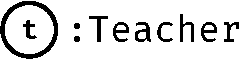
\includegraphics[height=2.6ex]{figures/subgraph-patterns/teacher_t.pdf}}}}
  \newcommand{\pfriendoft}{\vcenter{\hbox{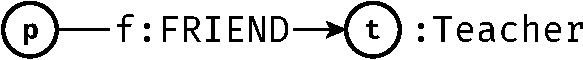
\includegraphics[height=2.6ex]{figures/subgraph-patterns/p_friend_teacher_t.pdf}}}}
  
  It holds that
  \[
    \expandin{t}{f:\{\text{FRIEND}\}}{p}(\result(\teachert)) = \result(\pfriendoft)
  \]
\end{example}


\begin{definition}[\op{LabelSelection} operator]
\label{def:label-selection}

The \op{LabelSelection} operator $\selection{v:l}(\Omega)$ takes a query
result $\Omega$ as input and returns only those subgraphs where the node
matched by $v$ has the label $l$.

It is defined as
\begin{align*}
  \selection{v:l}(\Omega) := \{ \mu \in \Omega \mid l \in \nlabel(\mu(v)) \}
\end{align*}

\begin{proofof}{\op{LabelSelection} is a well-defined operator.}
\label{proof:label-selection-well-defined}

Let $\Omega$ be a query result and
$\rho' = (V_{\rho'}, R_{\rho'}, \lambda_{\rho'}, \nlabel_{\rho'}, \rtype_{\rho'}, \rpairs_{\rho'})$
the corresponding subgraph pattern.

Let then $\rho = (V_\rho, R_\rho, \lambda_\rho, \nlabel_\rho, \rtype_\rho, \rpairs_\rho)$
with
\begin{itemize}[label={}]
  \item $V_\rho := V_{\rho'}$
  \item $R_\rho := R_{\rho'}$
  \item $\lambda_\rho := \lambda_{\rho'}$
  \item $\nlabel_\rho(x) := \begin{cases}
                              \nlabel_{\rho'} \union \{ l \}, \text{ if } x = v \\
                              \nlabel{\rho'}(x), \text{ otherwise}
                            \end{cases}$
  \item $\rtype_\rho := \rtype_{\rho'}$
  \item $\rpairs_\rho := \rpairs_{\rho'}$
\end{itemize}

Once more we have to show that every subgraph in
$\selection{v:l}(\Omega)$ is also in $\result(\rho)$ and vice
versa.

\begin{itemize}
  \item[$(\subseteq)$]
    Take $\mu \in \selection{v:l}(\Omega)$ arbitrary.
    Then $\mu \in \Omega$ with $l \in \nlabel(\mu(v))$.
    
    We show again that each constraint of Definition \ref{def:query-result} is
    fulfilled (but with less detail, to avoid repetition):
    \begin{enumerate}[(1)]
      \item % (1) Node variables are mapped to nodes and relationship variables
            % to relationships
        Fulfilled, because $\mu \in \Omega$ and $\Omega$ is a query result.
        
      \item % (2) Relationships between variables map to relationships in the
            %     database
        Fulfilled, because $\lambda_\rho = \lambda_{\rho'}$ and
        $\mu \in \result(\rho')$.
        
      \item % (3) The mapped nodes have at least the labels of the variables
        First of all, by definition $\{l\} \subseteq \nlabel(\mu(v))$.
        Also $\nlabel_{\rho'}(v) \subseteq \nlabel(\mu(v))$, because
        $\mu \in \Omega$ and $\Omega$ is a query result.
        Therefore, $\nlabel_\rho(v) = \{l\} \union \nlabel_{\rho'}(v)
                                    \subseteq \nlabel(\mu(v))$
      
      \item % (4) The mapped relationships are in the set of allowed types
        Fulfilled, because $\rtype_\rho = \rtype_{\rho'}$ and
        $\mu \in \result(\rho')$.
        
      \item % (5) Relationships are unique in each partition.
        Fulfilled, because and $\rpairs_\rho = \rpairs_{\rho'}$ and
        $\mu \in \result(\rho')$.
    \end{enumerate}
    
    As a result, $\mu \in \result(\rho)$.

  \item[$(\supseteq)$]
    Take $\mu \in \result(\rho)$ arbitrary.
    Then $\mu \in \result(\rho') = \Omega$, because the subgraph pattern $\rho$
    has a superset of the constraints of $\rho'$.
    
    Also $\nlabel_\rho(v) = \nlabel_{\rho'}(v) \union \{l\}
                          \subseteq \nlabel(\mu(v))$
    which implies that $l \in \nlabel(\mu(v))$.
    
    Therefore, $\mu \in \selection{v:l}(\Omega)$.
\end{itemize}

We have proven that $\selection{v:l}(\Omega) = \result(\rho)$ and conclude that
\op{LabelSelection} is a well-defined operator.
\end{proofof}
\end{definition}

\begin{definition}[\op{DistinctSelection} operator]
\label{def:distinct}

The \op{DistinctSelection} operator $\distinct{r}{s}(\Omega)$ takes a query
result $\Omega$ as input and returns only those subgraphs where the
relationships matched by the variables $r$ and $s$ are different.

It is defined as
\begin{align*}
  \distinct{r}{s}(\Omega) := \{ \mu \in \Omega \mid \mu(r) \not = \mu(s) \}
\end{align*}

\begin{proofof}{\op{DistinctSelection} is a well-defined operator.}
\label{proof:distinct-well-defined}

Let $\Omega$ be a query result and
$\rho' = (V_{\rho'}, R_{\rho'}, \lambda_{\rho'}, \nlabel_{\rho'}, \rtype_{\rho'}, \rpairs_{\rho'})$
the corresponding subgraph pattern.

Let then $\rho = (V_\rho, R_\rho, \lambda_\rho, \nlabel_\rho, \rtype_\rho, \rpairs_\rho)$
with
\begin{itemize}[label={}]
  \item $V_\rho := V_{\rho'}$
  \item $R_\rho := R_{\rho'}$
  \item $\lambda_\rho := \lambda_{\rho'}$
  \item $\nlabel_\rho := \nlabel_{\rho'}$
  \item $\rtype_\rho := \rtype_{\rho'}$
  \item $\rpairs_\rho := \rpairs_{\rho'} \union \{ \{ r,s \} \}$
\end{itemize}

Once more we have to show that every subgraph in
$\distinct{r}{s}(\Omega)$ is also in $\result(\rho)$ and vice
versa.

\begin{itemize}
  \item[$(\subseteq)$]
    Take $\mu \in \distinct{r}{s}(\Omega)$ arbitrary.
    Then $\mu \in \Omega$ with $\mu(r) \not = \mu(s)$.
    
    We show again that each constraint of Definition \ref{def:query-result} is
    fulfilled:
    \begin{enumerate}[(1)]
      \item % (1) Node variables are mapped to nodes and relationship variables
            % to relationships
        Fulfilled, because $\mu \in \Omega$ and $\Omega$ is a query result.
        
      \item % (2) Relationships between variables map to relationships in the
            %     database
        Fulfilled, because $\lambda_\rho = \lambda_{\rho'}$ and
        $\mu \in \result(\rho')$.
        
      \item % (3) The mapped nodes have at least the labels of the variables
        Fulfilled, because $\nlabel_\rho = \nlabel_{\rho'}$ and
        $\mu \in \result(\rho')$.
      
      \item % (4) The mapped relationships are in the set of allowed types
        Fulfilled, because $\rtype_\rho = \rtype_{\rho'}$ and
        $\mu \in \result(\rho')$.
        
      \item % (5) Relationship variables are mapped to different relationships
            %     if they are marked different
        By definition it holds that $\{r,s\} \in \rpairs_\rho$ and
        $\mu(r) \not = \mu(s)$.
        
        Take now $\{t,u\} \in \rpairs_\rho$ with $\{t,u\} \not = \{r,s\}$.
        Then $\{t,u\} \in \rpairs_{\rho'}$ and because $\mu \in \result(\rho')$
        it follows that $\mu(t) \not = \mu(u)$.
    \end{enumerate}
    
    As a result, $\mu \in \result(\rho)$.

  \item[$(\supseteq)$]
    Take $\mu \in \result(\rho)$ arbitrary.
    Then $\mu \in \result(\rho') = \Omega$, because the subgraph pattern $\rho$
    has a superset of the constraints of $\rho'$.
    Because $\{r,s\} \in \rpairs_\rho$, we have $\mu(r) \not = \mu(s)$.
    
    Therefore, $\mu \in \distinct{r}{s}(\Omega)$.
\end{itemize}

We have proven that $\distinct{r}{s}(\Omega) = \result(\rho)$ and conclude that
\op{DistinctSelection} is a well-defined operator.
\end{proofof}
\end{definition}

\section{Completeness}
\label{sec:completeness}

A set of operators is \emph{complete}, iff it is possible to produce the whole
result space of the corresponding algebra by chaining these operators.

We are interested in the set
\[
  \operators_c := \{ \getnodes{v}, \join, \traversevar{v}{r:T}{\alpha}{w},
                     \selection{v:l}, \distinct{r}{s} \} \subset \operators
\]

\begin{proofof}{$\operators_c$ is a complete set of operators w.r.t.
                $\resultspace$.}
  Let $\rho = (V_\rho, R_\rho, \lambda_\rho, \nlabel_\rho, \rtype_\rho, \rpairs_\rho)$ be a
  subgraph pattern. We have to show that there is a combination of query
  operators from $\operators_c$ producing $\result(\rho)$.
  
  First of all, because $V_\rho, R_\rho$ are finite, we can enumerate them in
  a sequence:
  \[
    V_\rho = \{ v_1, v_2, \ldots, v_\card{V_\rho} \}, ~~ R_\rho = \{ r_1, r_2, \ldots, r_\card{R_\rho} \}
  \]
  
  The same holds for all labels of a node variable $v_i \in V_\rho$
  \[
    \nlabel_\rho(v_i) = \{ l_{i,1}, l_{i,2}, \ldots, l_{i,\card{\nlabel_\rho(v_i)}} \}
  \]
  and for all pairs of relationships in $\rpairs_\rho$
  \[
    \rpairs_\rho = \{ \{r_{1,1}, r_{1,2}\}, \ldots, \{r_{\card{\rpairs_\rho},1}, r_{\card{\rpairs_\rho},2}\} \}
  \]
  
  We can now reuse some work done in the previous proofs, where we showed that
  the query operators are well-defined.
  For each operator we defined an output subgraph pattern in terms of the
  input subgraph patterns. The idea for the completeness proof is the
  following:
  We build a chain of query operators which we suppose to equal
  $\result(\rho)$. Then we use the mentioned pattern definitions to find a
  pattern $\rho'$ that produces the same query result as this chain.
  We will see that $\rho' = \rho$ and therefore
  $\result(\rho') = \result(\rho)$.
  
  Let us start to build the chain of operators.
  
  \begin{enumerate}
    \item % 1. Matching single nodes.
      We begin with the following query result: 
      \begin{align*}
        J_1 &:= \getnodes{v_1} \\
        J_i &:= \getnodes{v_i} \join J_{i-1}
          ~~\text{ for } i \in \{ 2, \ldots, \card{V_\rho} \}
      \end{align*}
      
      In Definition \ref{def:get-nodes} we found that,
      $J_1 = \getnodes{v_1}$ can be produced by a pattern that has only one node variable,
      no relationships and no type or label constraints.
      Using Definition \ref{def:node-join} we observe that, given a pattern $\rho_{i-1}$
      producing $J_{i-1}$, a pattern $\rho_i$ producing $J_i$ can be obtained by simply
      adding the variable $v_i$ to the set of nodes of $\rho_{i-1}$.
      All other components of $\rho_i$ equal those of $\rho_{i-1}$.
      
      Consequently, the following pattern $\rho_J$ having all node variables
      $V_\rho$ but no relationships, no type constraints and no label
      constraints will produce $J_\card{V_\rho}$:
      
      $\rho_J = (V_\rho, \emptyset, \emptyset \rightarrow {V_\rho}^2,
       V_\rho \rightarrow \emptyset,
       \emptyset \mapsto \powSet{\rtypes} \setminus \emptyset,
       \emptyset)$.
      
   \item % 2. Matching relationships:
      In the next step, we match relationships between the nodes in
      $J_\card{V_\rho}$.
      
      For a tuple $t = (t_1, t_2, \ldots, t_n)$ we denote the projection on the
      $i$'th component with $\pi_i(t) := t_i$.
      
      We construct a sequence of \op{Traverse} operators matching all
      relationships that exist in $\rho$:
      \begin{align*}
        R_0 &:= J_\card{V_\rho} \\
        R_i &:= \traverseout{\pi_1(\lambda_\rho(r_i))}{r_i:\rtype_\rho(r_i)}{
          \pi_2(\lambda_\rho(r_i))}(R_{i-1})
      \end{align*}
      
      Incrementing the parameter from $i-1$ to $i$ means to append a
      \op{Traverse} operator for relationship $r_i$ to $R_{i-1}$.
      According to the proof that \op{Traverse} is well-defined
      (cf. Definition \ref{def:traverse}), this is equivalent to adding the relationship $r_i$
      to the corresponding subgraph pattern, together with the type constraint.
      
      It is easy to see that, $R_\card{R_\rho} = \result(\rho_R)$ with
      $\rho_R = (V_\rho, R_\rho, \lambda_\rho,
       V_\rho \rightarrow \{ \emptyset \},
       \rtype_\rho,
       \rpairs_\rho)$.
      This pattern already equals $\rho$ in all components except the label
      function and the set of distinct relationship pairs.
      
    \item % 3. Selecting by labels
      In the second last step, we shrink the set of subgraphs by adding label constraints.
      
      We define
      \begin{align*}
        L_{0,0} &:= R_\card{R_\rho} \\
        L_{i,0} &:= L_{i-1, \card{\nlabel_\rho(v_i)}}
          ~~\text{ for } i \in \{ 1, \ldots, \card{V_\rho} \} \\
        L_{i,j} &:= \selection{v_i:l_{i,j}}(L_{i,j-1})
          ~~\text{ for } i \in \{ 1, \ldots, \card{V_\rho} \},
                         j \in \{ 1, \ldots, \card{\nlabel(v_i)} \}
      \end{align*}
      
      We are interested in
      $L := L_{\card{V_\rho}, \card{\nlabel_\rho(v_\card{V_\rho})}}$.
      As in the previous two steps, we iteratively construct a subgraph pattern
      which produces the same result, using the recursive definition from the
      proof that the \op{LabelSelection} operator is well-defined
      (cf. Definition \ref{def:label-selection}).
      
      Going from $L_{i,j}$ to $L_{i,j-1}$ means to append a \op{LabelSelection}
      for label $l_{i,j}$ on the node variable $v_i$.
      According to the proof that \op{LabelSelection} is well-defined
      (cf. Definition \ref{def:label-selection}), this is equivalent to adding a new label
      to $\nlabel(v_i)$ in the corresponding subgraph pattern.
      All other components of the pattern do not change.
      
      We see that $L$
      contains exactly one \op{LabelSelection} for each label constraint stored
      in $\nlabel_\rho$.
      Therefore, going from the previous pattern $\rho_R$ to a pattern $\rho_L$
      with $\result(\rho_L) = L$,
      means adding all of the label constraints from $\nlabel_\rho$ to
      $\rho_R$. Because there are no label constraints in $\rho_R$, the label
      function in $\rho_L$ simply equals $\nlabel_\rho$.
      
      Thus the generated pattern is
      \[
         \rho_L = (V_\rho, R_\rho, \lambda_\rho, \nlabel_\rho, \rtype_\rho, \emptyset)
      \]
      
    \item % 4. Selecting distinct relationships
      In the final step, we shrink the set of subgraphs by introducing
      constraints ensuring relationship uniqueness.
      
      We define
      \begin{align*}
        U_0 &:= L \\
        U_i &:= \distinct{r_{i,1}}{r_{i,2}}(U_{i-1})
          ~~\text{ for } i \in \{ 1, \ldots, \card{\rpairs_\rho} \}
      \end{align*}
      
      We are interested in $U := U_\card{\rpairs_\rho}$.
      We proceed as in the previous steps.
      
      Going from $U_i$ to $U_{i-1}$ means to append a \op{DistinctSelection} operator
      for the relationships $r_{i,1}, r_{i,2}$.
      According to the proof that \op{DistinctSelection} is well-defined
      (cf. Definition \ref{def:distinct}), this is equivalent to adding the pair
      $\{r_{i,1}, r_{i,2}\}$ to the set of distinct relationship pairs in the
      corresponding subgraph pattern.
      All other components of the pattern do not change.
      
      We see that $U$ contains exactly one \op{DistinctSelection} operator for each
      pair of relationship variables stored in $\rpairs_\rho$.
      Therefore, going from the previous pattern $\rho_L$ to $\rho_U$
      with $\result(\rho_U) = U$, means adding all of the pairs from
      $\rpairs_\rho$ to $\rho_L$.
      Because the set of distinct relationship pairs of $\rho_L$ is empty, the
      set of distinct relationship pairs of $\rho_U$ simply equals
      $\rpairs_\rho$.
      
      Thus the generated pattern is
      \[
         \rho_U = (V_\rho, R_\rho, \lambda_\rho, \nlabel_\rho, \rtype_\rho, \rpairs_\rho) = \rho
      \]
      
      It follows that
      \[
        U = \result(\rho_U) = \result(\rho) ~\text{.}
      \]
  \end{enumerate}
\end{proofof}

% \section{Graph query languages}
%
% \begin{definition}[Graph query language]
% Take  a finite set of graph query operators $O_L \subset \operators$.
%
% The corresponding query language 
% \end{definition}
